\appendix
\chapter{Questionários}

\section{How do you choose between different Ruby Gems}

\begin{enumerate}
  \item \hspace{1pt} Your GitHub username?

  \item \hspace{1pt} Do you develop software? (Mark all that apply)
  \begin{enumerate}
	\item \hspace{1pt} No, I don't
    \item \hspace{1pt} Yes, professionally
    \item \hspace{1pt} Yes, non-professionally -- e.g., pet projects, tinkering, ...
    \item \hspace{1pt} Yes, I contribute to one or more open source projects (irrespective of size)
  \end{enumerate}

  \item \hspace{1pt} How long have you been developing in Ruby?
    \begin{enumerate}
      \item \hspace{1pt} I don't
      \item \hspace{1pt} Less than a year
      \item \hspace{1pt} 1-2 years
      \item \hspace{1pt} 3-5 years
      \item \hspace{1pt} More than 5 years
    \end{enumerate}

  \item \hspace{1pt} When there is more than one gem available that would fulfill your needs -- how do you decide which Gem you use?

  \item \hspace{1pt} What are the most important things you consider when choosing a Gem?

  \item \hspace{1pt} Is there room for improvement over the tools you use for finding Gems?

  \item \hspace{1pt} Would you be willing to do a short Skype / Hangout call with us so we can learn more about your response?

  \item \hspace{1pt} Thanks so much for getting this far! Any questions, comments or concerns you'd like to tell us about?

\end{enumerate}

\section{Questionário de Avaliação da Ferramenta}
\begin{enumerate}
  
  \item \hspace{1pt} Você conhece alguma das gems mencionadas?
    \begin{enumerate}
		\item \hspace{1pt} Sim, uma
        \item \hspace{1pt} Sim, ambas
        \item \hspace{1pt} Não
	\end{enumerate}
    
  \item \hspace{1pt} Comente o que você conhecia sobre cada Gem
  
  \item \hspace{1pt} Algum participante mudou sua opinião a respeito de alguma das gems?
  	\begin{enumerate}
  		\item \hspace{1pt} Sim, um
        \item \hspace{1pt} Sim, ambos
        \item \hspace{1pt} Não
    \end{enumerate}
  
  \item \hspace{1pt} Comente sobre a sua escolha acima
  
  \item \hspace{1pt} A partir de agora, você...
    \begin{enumerate}
  		\item \hspace{1pt} Vai usar ambas as gems, de acordo com o contexto
        \item \hspace{1pt} Vai usar somente uma das gems
        \item \hspace{1pt} Não vai usar nenhuma das gems
    \end{enumerate}
  
  \item \hspace{1pt} Comente sobre a sua escolha acima
  
  \item \hspace{1pt} Comente sobre o que você achou da ferramenta		

\end{enumerate}

\chapter{Comparativo entre projetos do GitHub e indicações do Ruby Toolbox}

\begin{figure}[ht]
	\centering
    \caption{Comparativo entre \textit{Frameworks} de Testes}
    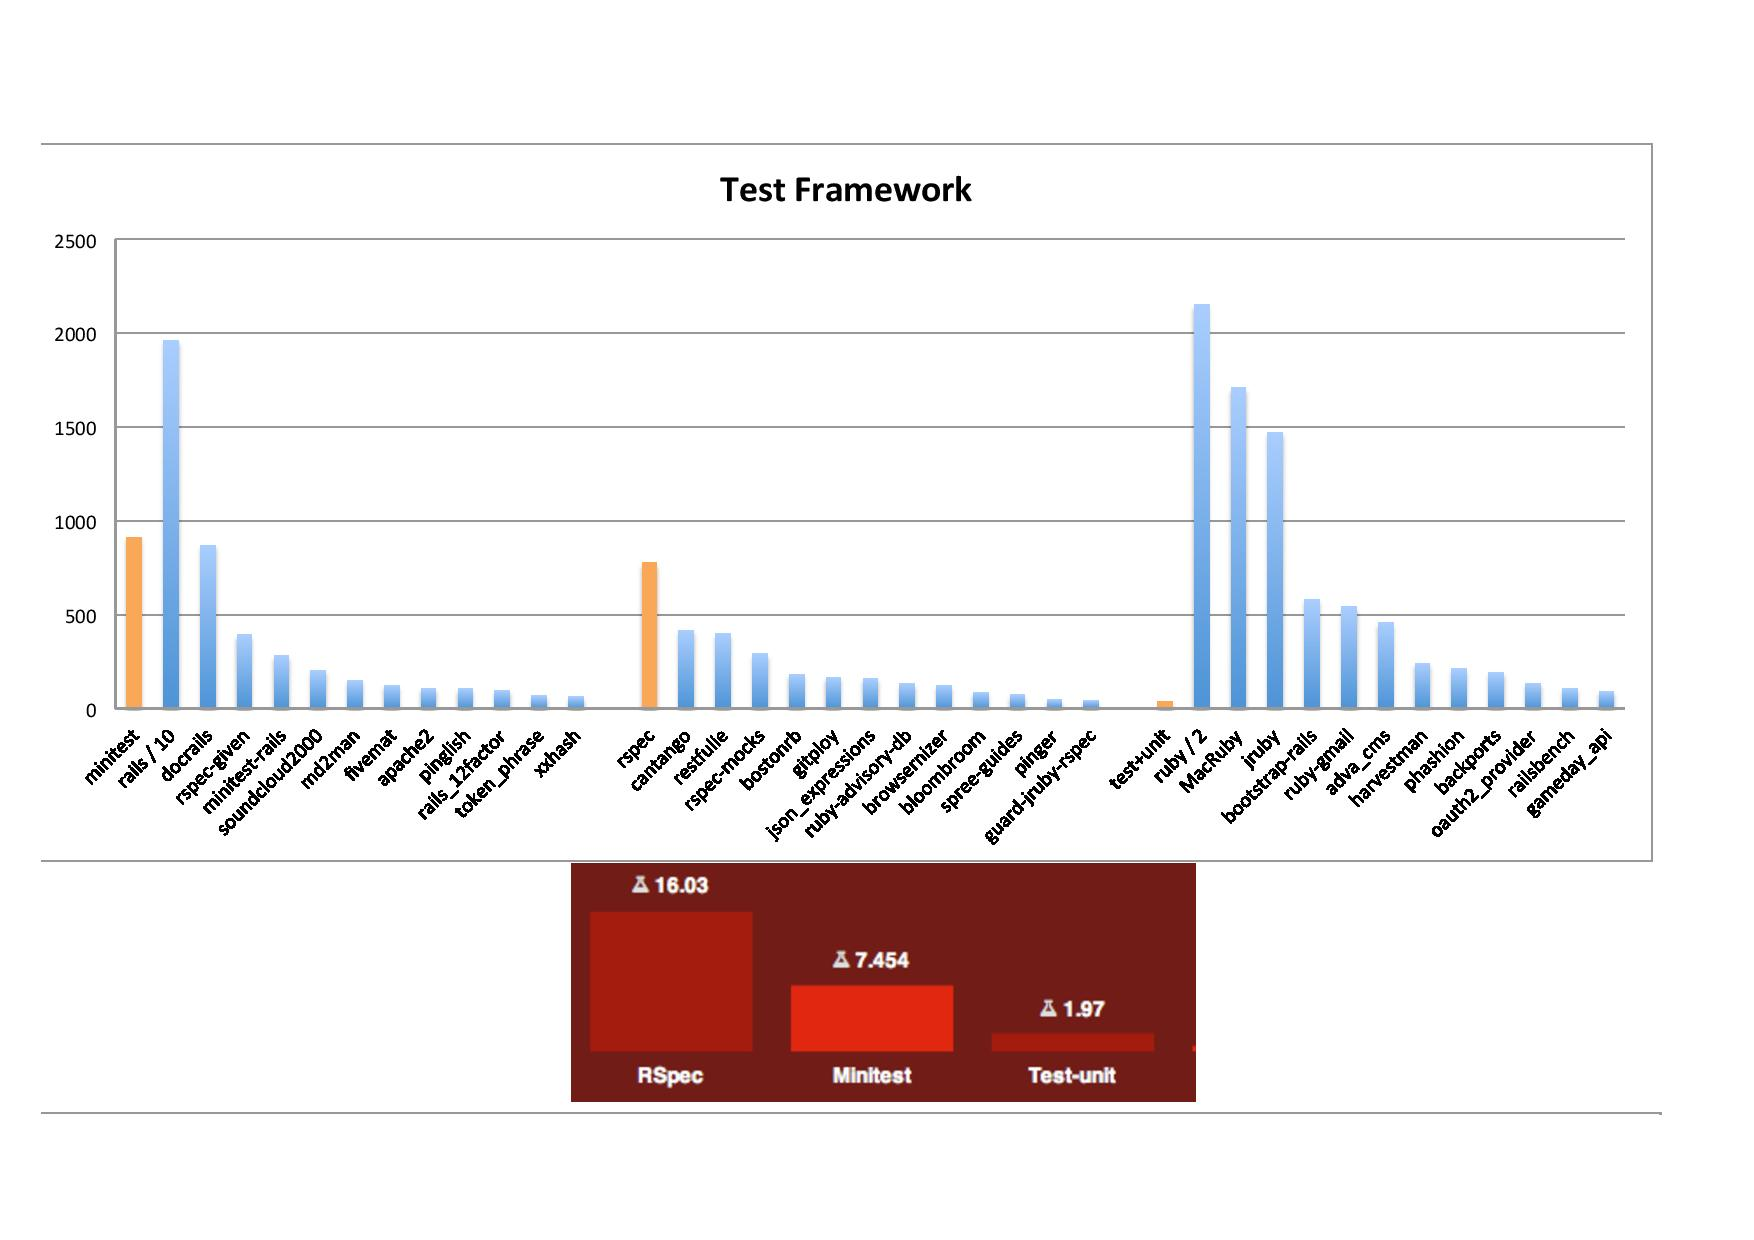
\includegraphics[width=15cm]{Imagens/gems-1.jpg}
	\caption*{Fonte: GitHub API e Ruby Toolbox (2013)}
\end{figure}
\begin{figure}[ht]
	\centering
    \caption{Rails \textit{Uploaders}}
    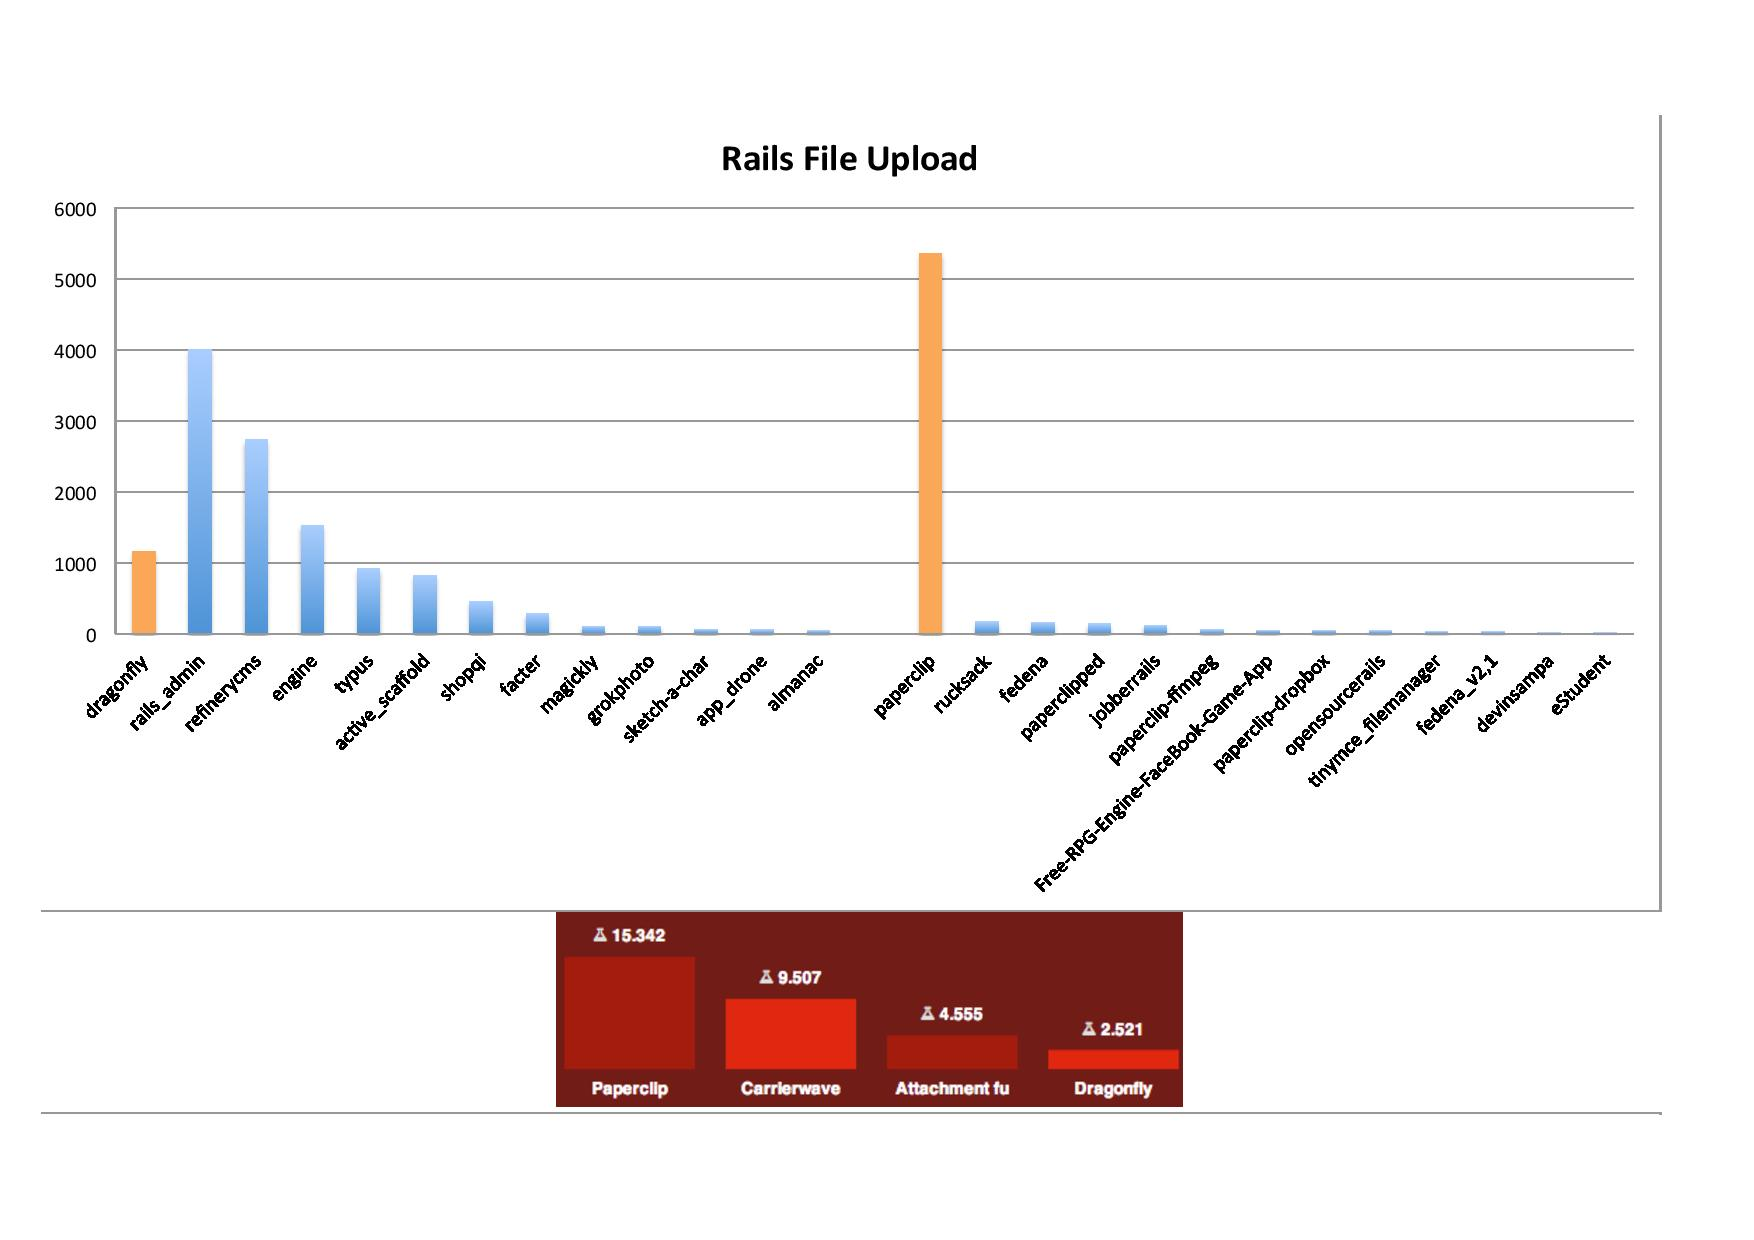
\includegraphics[width=15cm]{Imagens/gems-2.jpg}
	\caption*{Fonte: GitHub API e Ruby Toolbox (2013)}
\end{figure}
\begin{figure}[ht]
	\centering
    \caption{Clientes HTTP}
    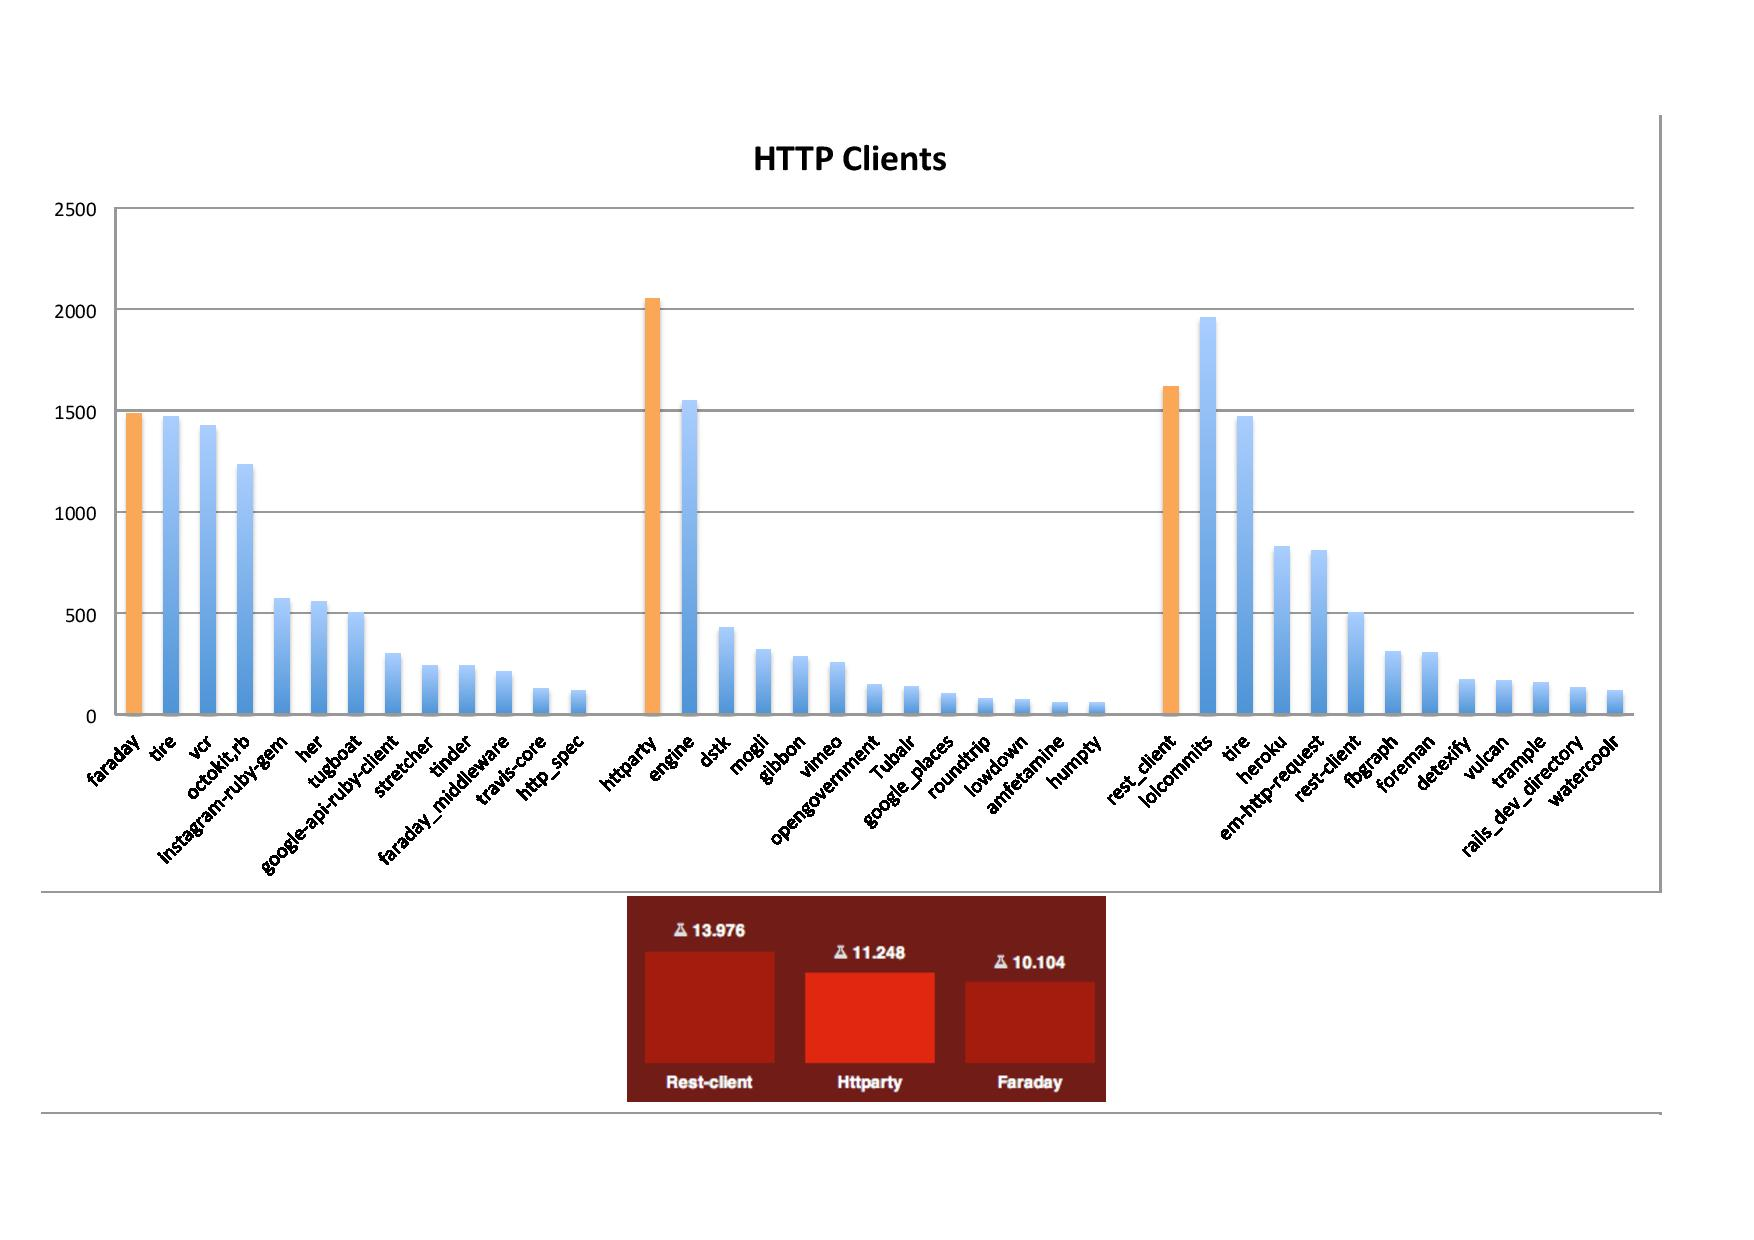
\includegraphics[width=15cm]{Imagens/gems-3.jpg}
	\caption*{Fonte: GitHub API e Ruby Toolbox (2013)}
\end{figure}
\begin{figure}[ht]
	\centering
    \caption{Construtores de Formulários}
    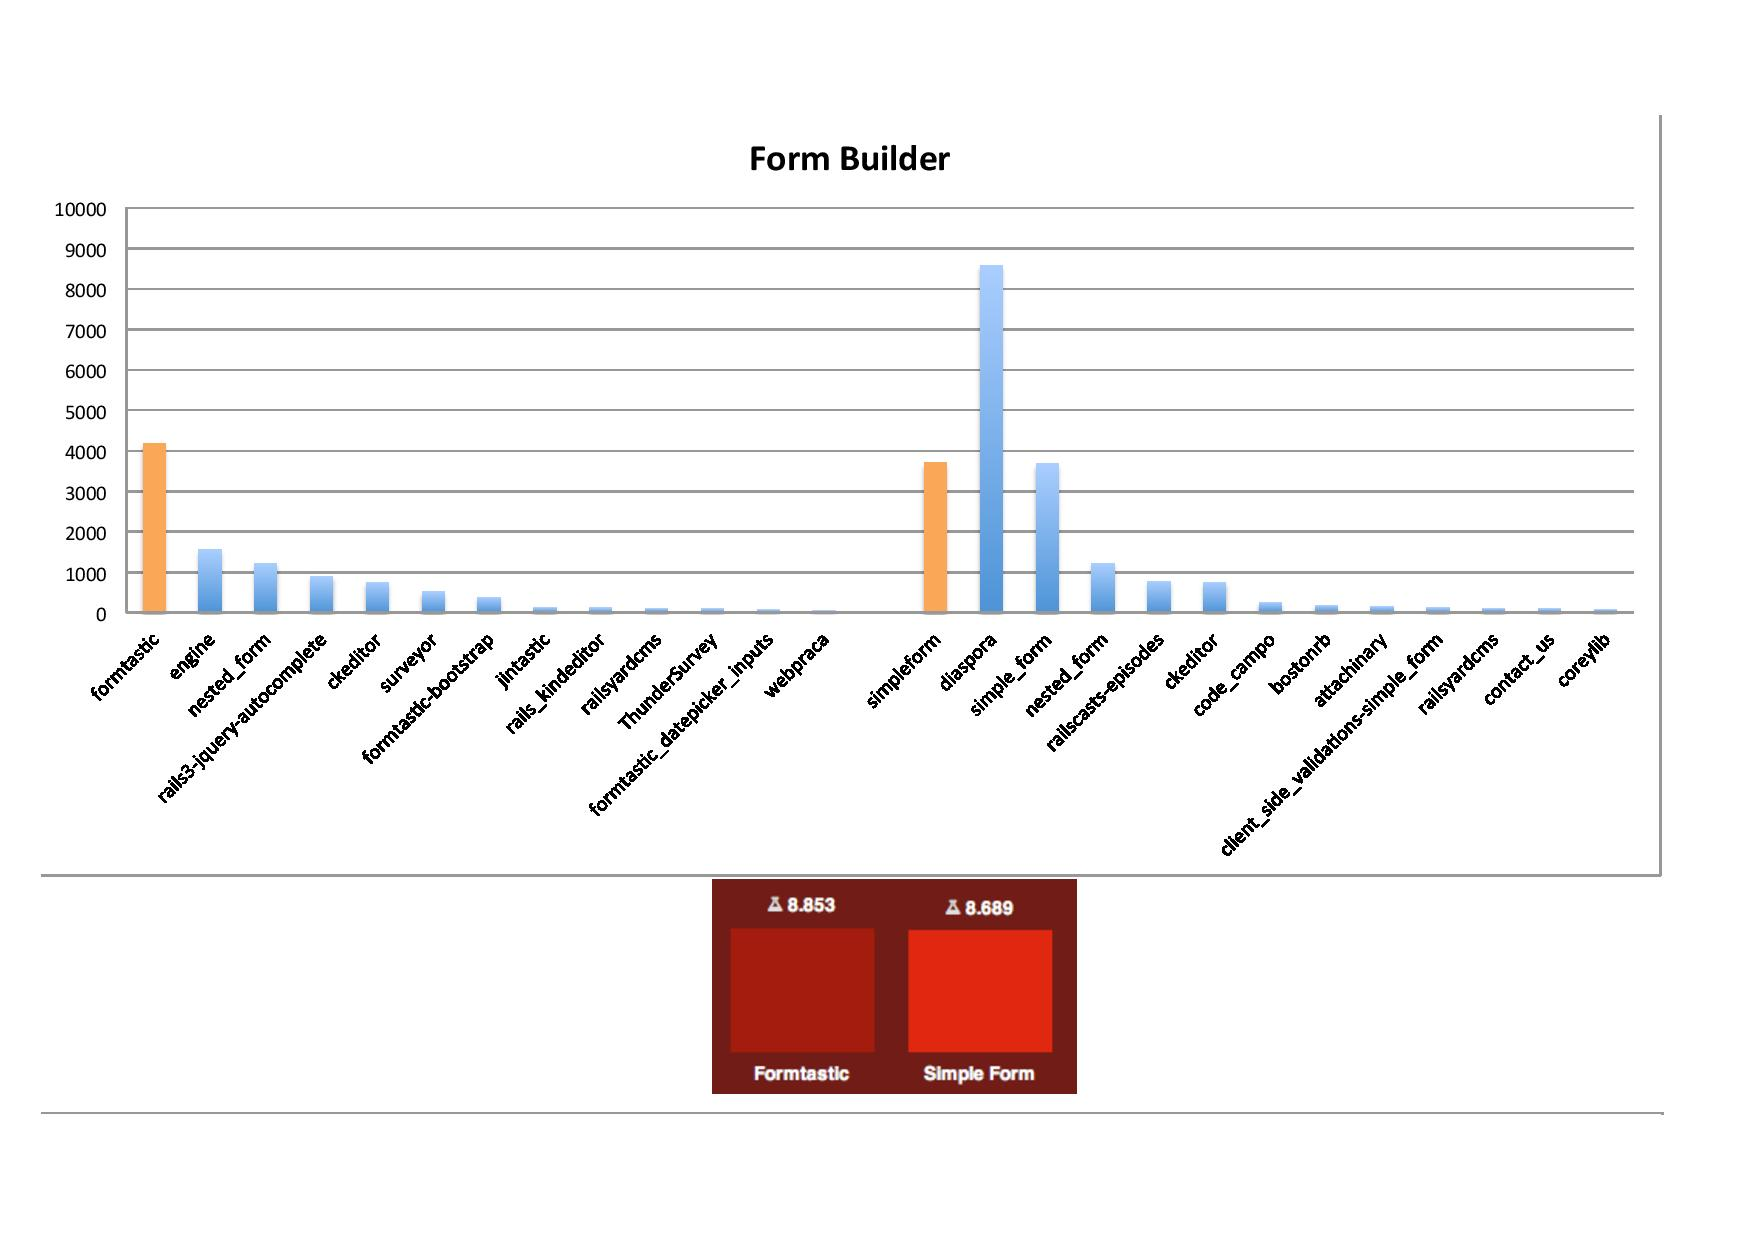
\includegraphics[width=15cm]{Imagens/gems-4.jpg}
	\caption*{Fonte: GitHub API e Ruby Toolbox (2013)}
\end{figure}
\begin{figure}[ht]
	\centering
    \caption{Interpretador de JSON}
    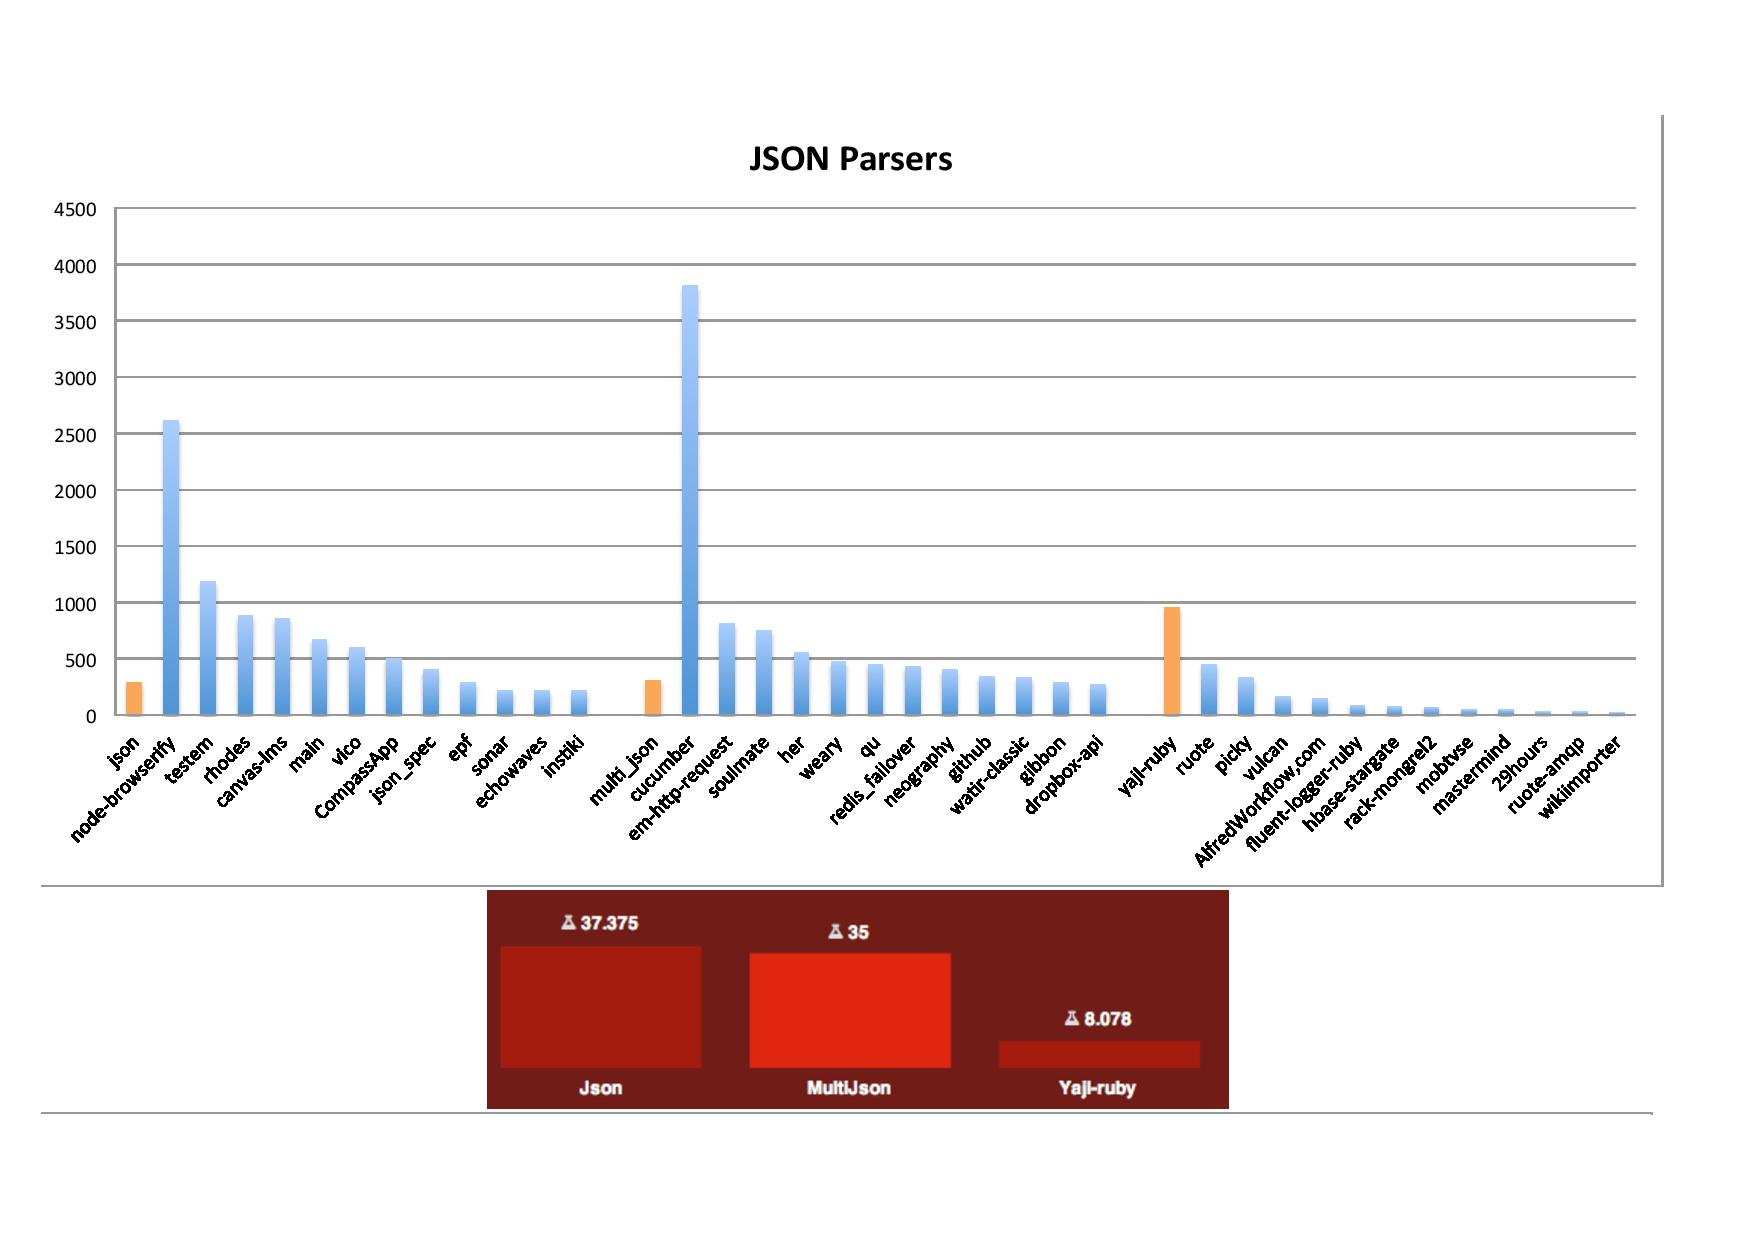
\includegraphics[width=15cm]{Imagens/gems-5.jpg}
	\caption*{Fonte: GitHub API e Ruby Toolbox (2013)}
\end{figure}
\begin{figure}[ht]
	\centering
    \caption{\textit{Template Engine}}
    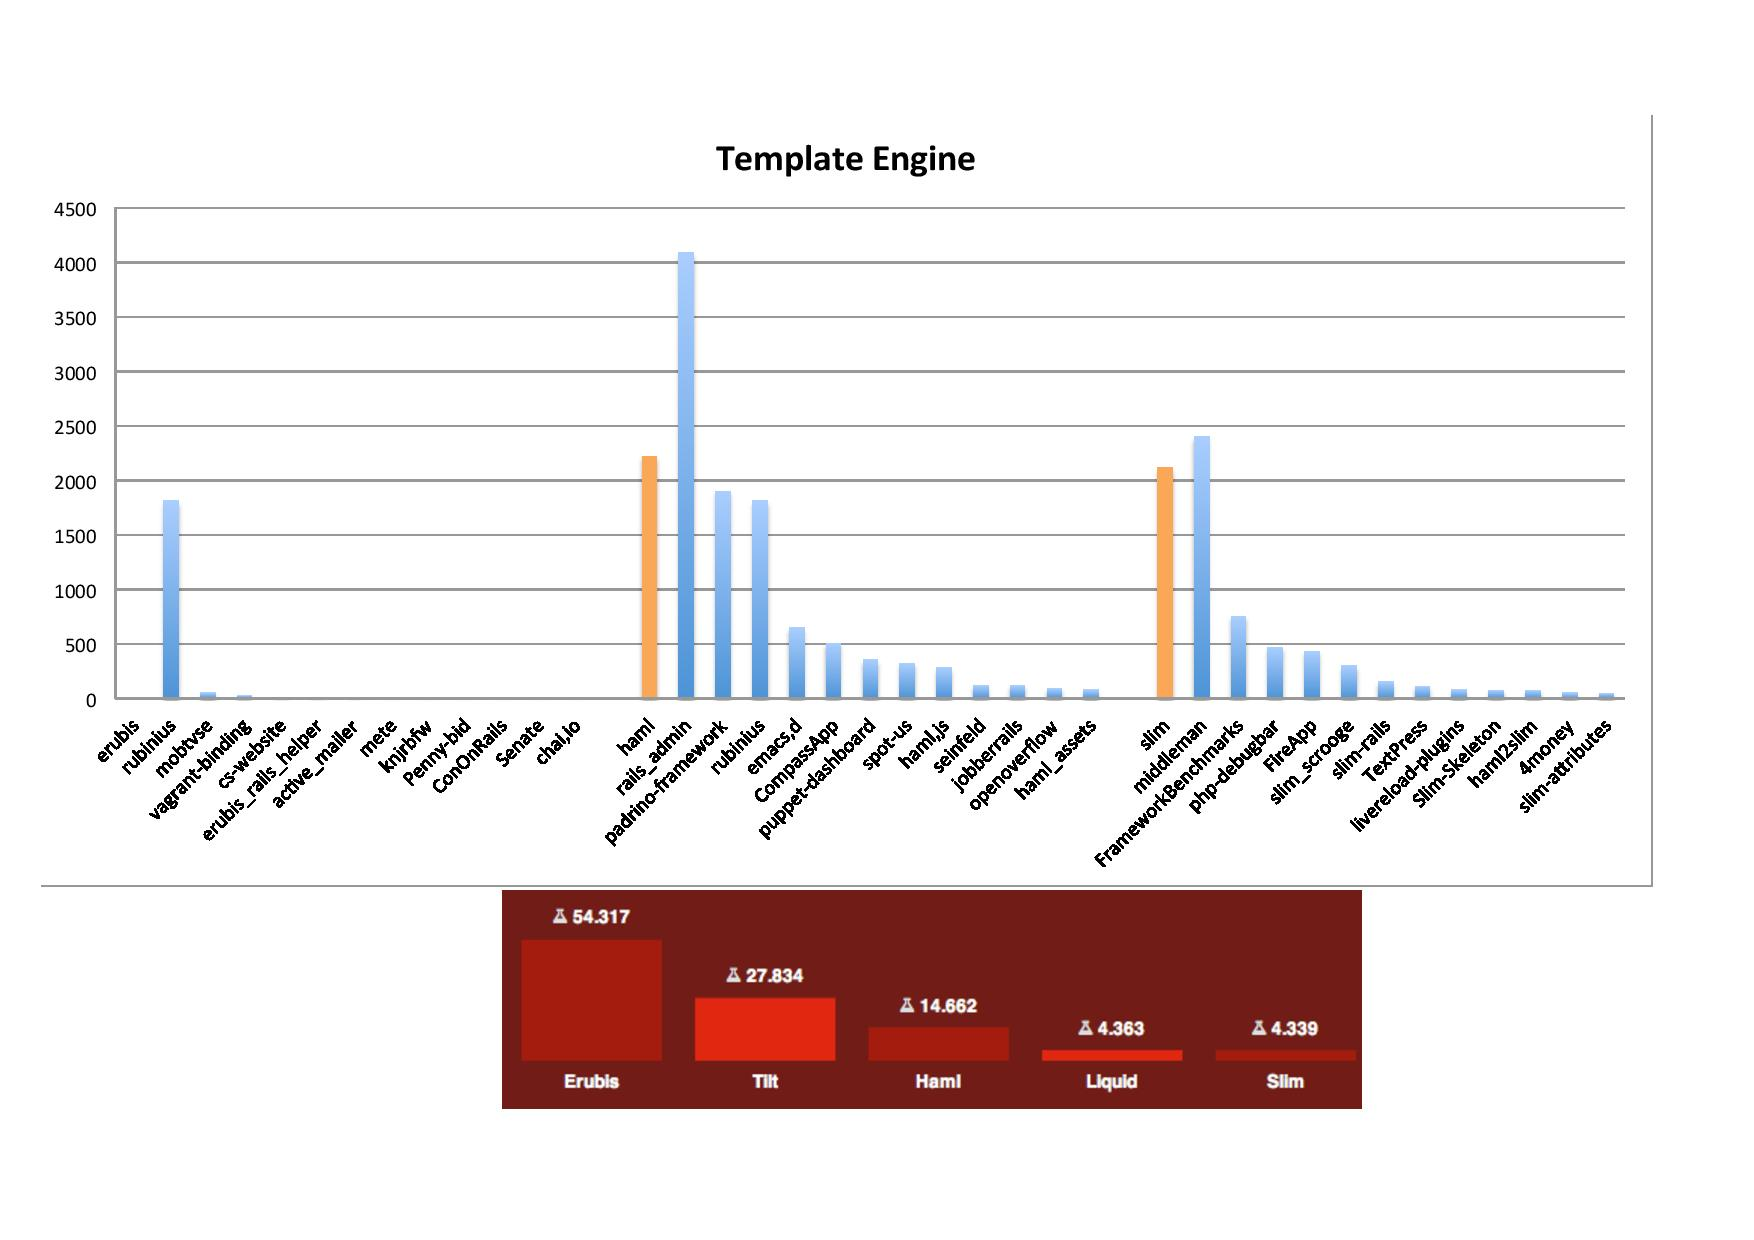
\includegraphics[width=15cm]{Imagens/gems-6.jpg}
	\caption*{Fonte: GitHub API e Ruby Toolbox (2013)}
\end{figure}